\documentclass{article}

\usepackage[accepted]{icml2024}

\usepackage{datetime}
\usepackage{amsfonts}
\usepackage{amsmath}
\usepackage{booktabs} % for professional tables

\usepackage{graphicx}
\usepackage{subcaption}

\usepackage{hyperref}

\begin{document}

\twocolumn[
\icmltitle{Learning Neural Orientation Field for Volumetric Hair Reconstruction}

% It is OKAY to include author information, even for blind
% submissions: the style file will automatically remove it for you
% unless you've provided the [accepted] option to the icml2024
% package.

% List of affiliations: The first argument should be a (short)
% identifier you will use later to specify author affiliations
% Academic affiliations should list Department, University, City, Region, Country
% Industry affiliations should list Company, City, Region, Country

% You can specify symbols, otherwise they are numbered in order.
% Ideally, you should not use this facility. Affiliations will be numbered
% in order of appearance and this is the preferred way.
\icmlsetsymbol{equal}{*}

\begin{icmlauthorlist}
\icmlauthor{Fangjun Zhou}{}
\icmlauthor{Zhenyu Zhang}{}
\icmlauthor{Weiran Xu}{}
\end{icmlauthorlist}

\icmlcorrespondingauthor{Fangjun Zhou}{fzhou48@stanford.edu}
\icmlcorrespondingauthor{Zhenyu Zhang}{zhenyuz5@stanford.edu}
\icmlcorrespondingauthor{Weiran Xu}{weiran@stanford.edu}

% You may provide any keywords that you
% find helpful for describing your paper; these are used to populate
% the "keywords" metadata in the PDF but will not be shown in the document
\icmlkeywords{Machine Learning, ICML, NeRF, MVS}

\vskip 0.3in
]

\begin{abstract}
    Reconstructing 3D human hair is challenging due to its intricate, intertwined structure and fine details. We propose Neural Orientation Field (NeOF) model that directly encodes hair’s growing direction and occupancy in 3D. Unlike conventional NeRF-based methods that rely on view-dependent radiance fields, our representation is view-independent and trained end-to-end from multiview 2D orientation maps. A novel volumetric renderer using differentiable projection of world-space orientations into screen-space, allowing supervision from multiple viewpoints. Experiments on synthetic datasets show that our approach recovers finer hair structures than baselines, establishing a robust, high-fidelity representation that can guide generative models or produce strand geometry directly.
\end{abstract}

\section{Introduction}

% Project motivation

Reconstructing human hair is one of the most challenging yet critical process in rendering photorealistic digital human. Unlike other parts of the human body, human hair is highly detailed and often intertwined together. Therefore, it's difficult to use traditional photogrammetry method to reconstruct its structure.

Before machine learning model is used in this field, artists often hand crafted splines on skulls to represent hair strands. Each strand is then textured and rendered to mimic the hair volume. This workflow requires a lot of experience as it's non-trivial for artists to infer the final render result from hair stand splines. To reduce the workload and improve the accuracy of hair reconstruction, machine learning models are trained to generate hair strand from captured images.

In this work, we propose a new method capturing the hair structure by learning a 3D orientation field from $\mathbb{R}^{3} \rightarrow \mathbb{R}^{2}$ representing the hair growing direction. On top of that, another occupancy field from $\mathbb{R}^{3} \rightarrow \mathbb{R}^{2}$ is learned to indicate hair and body occupancy. These mappings can be used later to generate hair strand directly by numerically integrating the orientation field. It can also be used as a latent variable to guide other generative models as mentioned in \cite{metzer_latent-nerf_2022}.

%% TODO: Include the input and output of the model. DONE

Our algorithm fits the 3D orientation field by a simple MLP model. The input of this model is a sample position in space, and the model predicts the hair orientation and occupancy at the sampled position. We also propose a volumetric renderer for orientation fields capable of rendering the 2D hair orientation map for unseen views. Since this volumetric rendering algorithm is differentiable, we are able to train the model on multiple 2D hair orientation map from different viewing angles.

\section{Related Work}

Previous attempts to 3D hair reconstruction mainly focused on learning-based hair strand generation. This includes some studies about single view hair synthesis \cite{saito_3d_2018, zheng_hairstep_2023, wu_neuralhdhair_2022, ma_single-view_nodate}. Since the image only contains hair structure from one viewing angle, it's impossible to reconstruct entire hair accurately. These models often use pretrained image encoders such as ResNet-50 \cite{saito_3d_2018} to encode the abstract hair style into a feature vector, then use generative models such as U-Net \cite{zheng_hairstep_2023}, VAE \cite{saito_3d_2018}, and diffusion models \cite{sklyarova_neural_2023} to generate the final strand.

% In \cite{sklyarova_neural_2023} and \cite{rosu_neural_2022}, the authors also tried hair syntheses from multi-view images. However, these two studies still failed to capture finer details.

Another study about this topic tried expanding the traditional PatchMatch MVS (PMVS) algorithm to a Line-based PatchMatch MVS (LPMVS) \cite{nam_strand-accurate_nodate}. This method, despite its high accuracy, doesn't capture the volumetric property of human hair.

Our work is highly inspired by NeRF \cite{mildenhall_nerf_2020}, a model used for 3D reconstruction from 2D images. However, our model differs in two major way.

In NeRF, the model fits a radiance field from $\mathbb{R}^{5} \rightarrow \mathbb{R}^{4}$. The input of the radiance function includes the sample position and camera ray direction. However, since the orientation field our model fits is view-independent, the input space is only $\mathbb{R}^{3}$. This makes it easier for the model to capture more information from a smaller dataset.

On top of that, the volumetric renderer on orientation field also differs from the one on radiance field. When sampling the radiance field, NeRF only integrates the sampled color for each ray, while our model needs to project the sample orientation onto the filming plane and then integrate the projected orientation.


\section{Dataset}

%% TODO: Data generation. (Fangjun) DONE

The dataset used by this project is generated by a Blender geometry node-based hair system demo file \cite{foundation_blender_nodate}. We render the model from multiple viewing angles and exported the camera intrinsics and extrinsics for later use.

Each instance includes a ray-traced image rendered by Cycles renderer, a body mask, a hair mask, and a screen space hair orienrtation map (Figure~\ref{fig:dataset}). The screen space hair orienrtation map stores the projected hair orientation in red and green channel. To render this map, we calculated the world space hair orientation with a custom geometry node and rendered the screen space orientation with a custom shader and Blender's AOV render pass.

Our training set consists of 128 instances and our test set consists of 16 instances, all rendered from the same model but with different camera poses.

\begin{figure}[h]
	\centering
	\begin{subfigure}{0.11\textwidth}
		\centering
		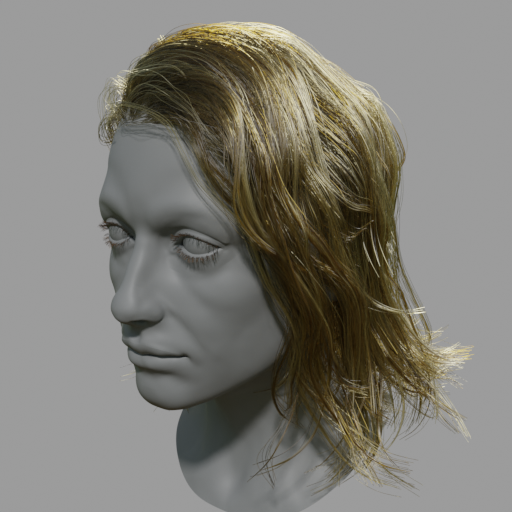
\includegraphics[width=\textwidth]{./images/dataset/0009_rendered.png}
		\caption{rendered}
	\end{subfigure}
	\hfill
	\begin{subfigure}{0.11\textwidth}
		\centering
		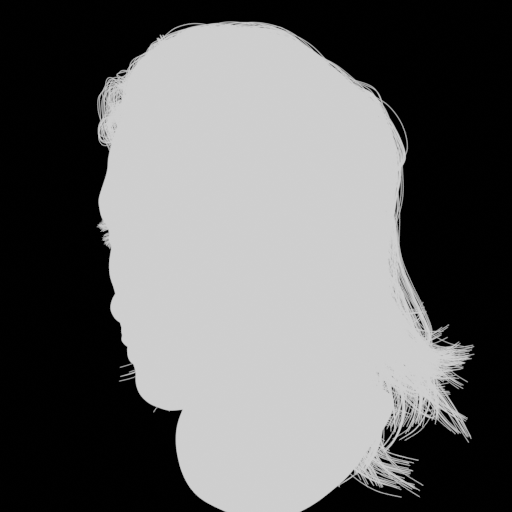
\includegraphics[width=\textwidth]{./images/dataset/0009_bodymask.png}
		\caption{body mask}
	\end{subfigure}
	\hfill
	\begin{subfigure}{0.11\textwidth}
		\centering
		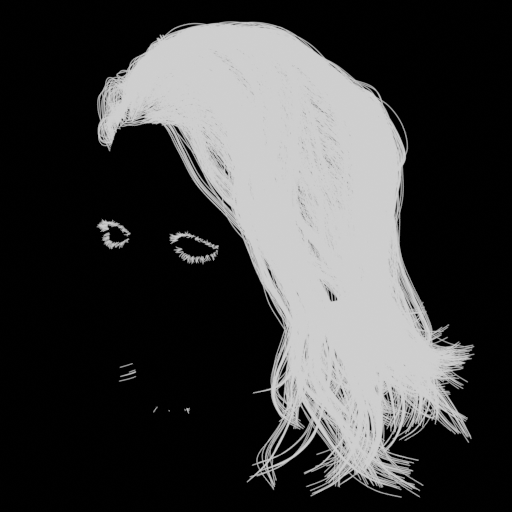
\includegraphics[width=\textwidth]{./images/dataset/0009_hairmask.png}
		\caption{hair mask}
	\end{subfigure}
	\hfill
	\begin{subfigure}{0.11\textwidth}
        \centering
        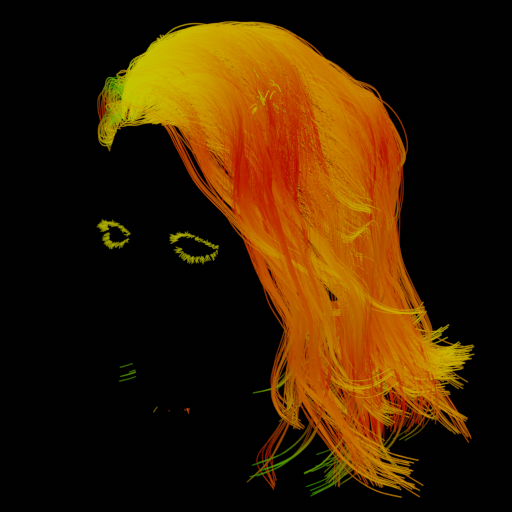
\includegraphics[width=\textwidth]{./images/dataset/0009_hairdir.png}
        \caption{orientation}
	\end{subfigure}

	\caption{Synthetic dataset rendered by Blender}
	\label{fig:dataset}
\end{figure}

\section{Method}

% TODO: Model structure. (Fangjun) DONE
% TODO: Volumetric renderer for vector field. (Fangjun) DONE
% TODO: Occupancy integration and mask loss. (Fangjun) DONE

\subsection{Neural Orientation Field (NeOF) Model}

The neural orientation field (NeOF) model we propose consists of multiple MLP layers and residual connections. The input of the network is the spatial coordinates $(x, y, z)$ of the point to be sampled. The output is the world space hair orientation $(\theta, \phi)$, as well as the opacity parameter $\sigma = (\sigma_{hair}, \sigma_{body})$.

\subsection{Volumetric Rendering for Neural Orientation Field}

As the training data only consists of screen space hair orientation. We propose a differentiable volumetric renderer $VolumetricRenderer(O_{world}, \Sigma)$ to render screen space hair orientation as well as body/hair masks from sampled world space orientation $O_{world} = \{ \mathbf{o}_{world}^{(i)} \}$ and occupancy $\Sigma = \{ \sigma^{(i)} \}$. To sample $O_{world}$ and $\Sigma$ for a pixel, we emit a camera ray with the known camera intrinsics and extrinsics on the filming plane. Then, the world space hair orientation and occupancy can be sampled along the camera ray. The volumetric rendering pipeline first projects the world space orientation to screen space, then integrate the screen space orientation with the sampled occupancy.

To project hair orientation, we first need to convert the world space orientation $\mathbf{o}_{world}$ to an orientation vector in homogeneous coordinate $\mathbf{v}_{world} \in \mathbb{R}^{4}$. Given the camera extrinsic matrix $M \in \mathbb{R}^{4 \times 4}$, $\mathbf{v}_{world}$ can be projected to the view space by $\mathbf{v}_{view} = M\mathbf{v}_{world}$.

Normally, to project a world space vector onto screen space, we need to first apply view transform to get view space projection, then apply perspective transform to get screen space projection. However, as we choose pinhole camera as our camera model, the screen space orientation vectors are independent of the camera intrinsics. In other words, $\mathbf{v}_{screen} = \mathbf{v}_{view} = M\mathbf{v}_{world}$

Similar to the volumetric rendering function defined in NeRF \cite{mildenhall_nerf_2020}, our rendering function for screen space orientation can be written as

\begin{align}
	V(\mathbf{r}) & = \int_{t_{n}}^{t_{f}} T(t) \sigma_{hair}(\mathbf{r}(t)) M \mathbf{v}_{world}(\mathbf{r}(t)) dt \\
	T(t) & = exp(-\int_{t_{n}}^{t} \sigma_{body}(\mathbf{r}(s)) ds)
\end{align}

One important difference between our model and NeRF is we use two separate occupancy for body and hair, while in NeRF only one occupancy is used to integrate camera rays. In our case, camera rays can be blocked by face and body that doesn't contribute to the final integration. Therefore, we use $\sigma_{body}$ instead of $\sigma_{hair}$ to integrate residual ray $T(t)$.

As we provide body mask and hair mask in the training data, we can also use the following rendering function to render body mask $B(\mathbf{r})$ and hair mask $H(\mathbf{r})$:

\begin{align}
	B(\mathbf{r}) & = 1 - exp(-\int_{t_{n}}^{t_{f}} \sigma_{body}(\mathbf{r}(s)) ds) \\
	H(\mathbf{r}) & = 1 - exp(-\int_{t_{n}}^{t_{f}} \sigma_{hair}(\mathbf{r}(s)) ds)
\end{align}

Similar to the numerical estimation of radiance integration mentioned in NeRF, we use numerical estimation of orientation and mask integration defined as follows:

\begin{align}
	\hat{V}(\mathbf{r}) & = \sum_{i=1}^{N} T_{i} (1 - exp(-\sigma_{hair}^{(i)} \delta_{i})) M \mathbf{v}_{world}^{(i)} \\
	T_{i} & = exp(-\sum_{j=1}^{i} \sigma_{body}^{(j)} \delta_{j}) \\
	\hat{B}(\mathbf{r}) & = 1 - exp(-\sum_{i=1}^{N} \sigma_{body}^{(i)} \delta_{i}) \\
	\hat{H}(\mathbf{r}) & = 1 - exp(-\sum_{i=1}^{N} \sigma_{hair}^{(i)} \delta_{i})
\end{align}

where $\delta_{i} = t_{i + 1} - t_{i}$. $\hat{V}(\mathbf{r})$, $\hat{B}(\mathbf{r})$, and $\hat{H}(\mathbf{r})$ are the final outputs of our volumetric render. The final loss is defined as the sum of orientation loss and mask losses. In theory, only orientation loss is required for the model to converge. However, we observed that introducing the mask losses helps improving the convergence speed. It also improves the model's performance on occupancy prediction accuracy.

\section{Experiment}

% TODO: Hierachical volumetric sampling for vector field. (Fangjun) DONE
% TODO: Experiement setup. (Fangjun, Zhenyu) DONE
% TODO: Implementation Details. (Fangjun) DONE
% TODO: Baseline setup. DONE

\subsection{Implementation Details}

\subsubsection{Position Encoding and Hierarchical Volume Sampling}

We use position encoding and hierarchical volume sampling mentioned in \cite{mildenhall_nerf_2020} to improve convergence rate in our implementation.

The position encoding function is defined as:

\begin{align}
    \gamma(p)_{2i} &= sin(2^{i} \pi p) \\
    \gamma(p)_{2i + 1} &= cos(2^{i} \pi p)
\end{align}

As mentioned in \cite{mildenhall_nerf_2020}, deep neural networks tend to fit low frequency functions. Using position encoding functions helps improve the convergence rate on high frequency data. This is extremely important for our application as the spatial frequency of hair orientation and occupancy is very high. In our experiment, at least 8 levels of position encoding is required to capture detailed hair directions.

For hierarchical volume sampling, we trained a coarse and a fine model simultaneously to fit the scene. The coarse model is used with an even sample depth to render the orientation map. The sampled body occupancy is then used to generate subdivided sample depth for the fine model. Areas with higher body occupancy in the coarse model will receive higher sample rate when rendered with the fine model. As mentioned previously, due to the high frequency nature of hair structure, hierarchical volume sampling is also always required in practice.

\subsubsection{NeOF Model Training and Test Setup}

Our model is trained on a training set of 128 2D orientation maps of size 512x512. We use Adam optimizer with $2e-4$ learning rate. For the coarse model, we use 6 levels of position encoding with a fixed sample rate of 16. For the fine model, we use 8 levels of position encoding with the maximum subdivided sample rate of 8. The model is trained for 8 epochs and the checkpoint with lowest loss on validation set is save.

\subsection{Metrics}

To evaluate the performance of the model, we rendered the orientation field on 16 unseen camera views in the test set and evaluate the performance using rendered 2D orientation.

We use MSE (Mean Squared Error) and PSNR (Peak Signal-to-Noise Ratio) for evaluation. The reconstructed 2D hair orientation map is compared with the ground truth 2D hair orientation by calculating the MSE, and the MSEs from all different viewpoints are averaged. This average MSE is then used to compute the overall PSNR metric. The complete formula is as follows:

\begin{align}
    \text{MSE}_k &=
    \frac{1}{M \cdot N \cdot 2}
     \sum_{i=1}^M \sum_{j=1}^N \| I_k (i,j) - K_k(i,j)\|_2 ^2 \\
    \text{MSE}_\text{avg} &= \frac{1}{N_\text{images}} \sum_{k=1}^{N_\text{images}}\text{MSE}_k \\
    \text{PSNR}_\text{avg} &= 10 \cdot \log_{10} \left( \frac{\text{MAX}^2}{\text{MSE}_{\text{avg}}} \right)
\end{align}

where $\text{MSE}_k$ is the MSE of image $k$ and its ground truth, $I_k$ and $K_k$ are the reconstructed 2D hair orientation for image $k$, $N$ and $M$ is the height and weight of the image, $N_\text{images}$ is the number of images, $\text{MSE}_\text{avg}$ is the average MSE of these image, MAX is the maximum possible value of each pixel (here we use 8-bit image, so it is 255), and $\text{PSNR}_\text{avg}$ is our final PSNR value.

\subsection{Baseline Method}

We choose NeRF \cite{mildenhall_nerf_2020} and HairStep \cite{zheng_hairstep_2023} as our baseline models. Since NeRF does not inherently encode hair orientation, and the HairStep model uses single view images to predict screen space hair orientation directly, we trained the NeRF model on rendered images to fit the radiance field. For each unseen views in the testing set, we first rendered colored images with the NeRF model. Then, we used the HairStep model to predict the screen space orientation on the rendered image. We also ran HairStep inference without NeRF to evaluate it's single view performance.

Observed that the output of NeRF is often blurred, consistent with findings from the original NeRF paper \cite{mildenhall_nerf_2020}, which noted that NeRF tends to capture low-frequency features early in training, making HairStep difficult to segment out hair and output reasonable hair direction, thus unable to maintain relevant direction information; see Figure \ref{fig:nerf_hairstep}.

\begin{figure}[h]
    \centering
    \begin{subfigure}{0.22\textwidth}
        \centering
        \begin{subfigure}{0.48\textwidth}
            \centering
            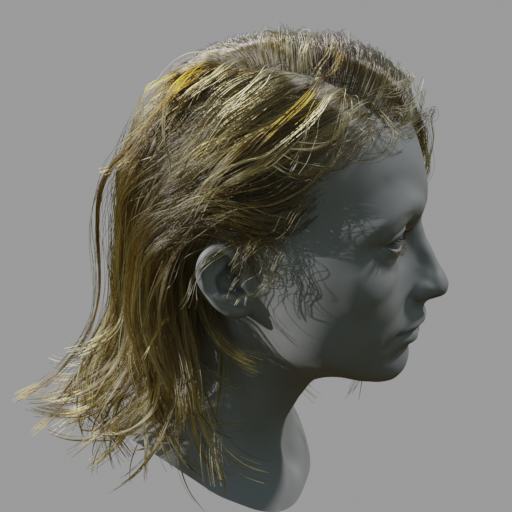
\includegraphics[width=\textwidth]{./images/baseline-method/test_6_rendered.png}
        \end{subfigure}
        \hfill
        \begin{subfigure}{0.48\textwidth}
            \centering
            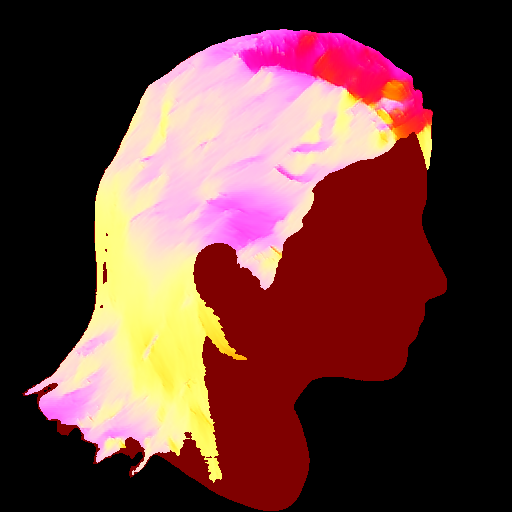
\includegraphics[width=\textwidth]{./images/baseline-method/test_6_hairstep.png}
        \end{subfigure}
        \caption{HairStep}
    \end{subfigure}
    \hfill
    \begin{subfigure}{0.22\textwidth}
        \begin{subfigure}{0.48\textwidth}
            \centering
            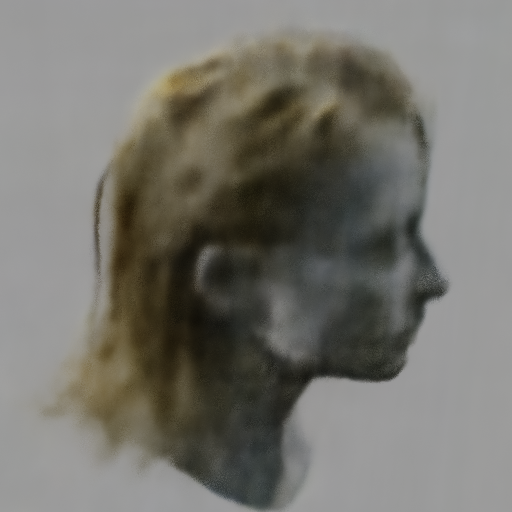
\includegraphics[width=\textwidth]{./images/baseline-method/pred_6_nerf.png}
        \end{subfigure}
        \hfill
        \begin{subfigure}{0.48\textwidth}
            \centering
            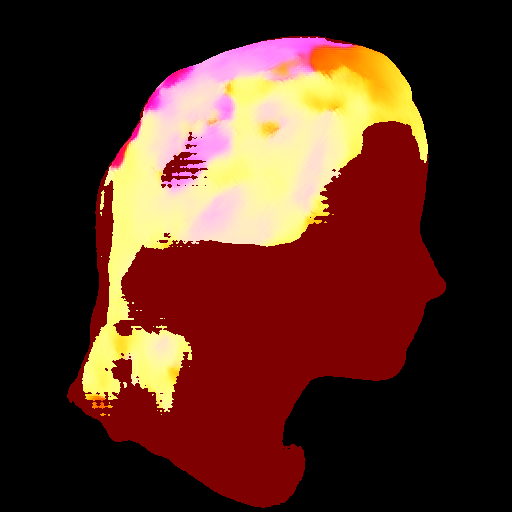
\includegraphics[width=\textwidth]{./images/baseline-method/pred_6_hairstep.png}
        \end{subfigure}
        \caption{NeRF with HairStep}
    \end{subfigure}

    \caption{Hairstep on rendered image/NeRF prediction}
    \label{fig:nerf_hairstep}
\end{figure}

Another difference between HairStep and our method is that HairStep predicts normalized hair orientation while our method captures the screen space projection of the world space hair orientation, which is not normalized. This means a hair strand growing perpendicular or parallel to the filming plane may have the same orientation in HairStep prediction. In contrast, our model will generate orientation vector with smaller magnitude for perpendicular strands.

To evaluate the performance of both models with the same metrics, we normalized the ground truth and NeOF output before evaluation.

\section{Result and Discussion}


By comparing our method with the two baselines, HairStep and NeRF, we can observe from the evaluation metrics PSNR and MSE that our results outperform the two baselines. The result shows in Table \ref{tab:loss_comparison}. Sample images are shown in Figure \ref{fig:result_grid}. We represent the direction of planar hair at a given point using vectors formed by the red and green channels of the RGB images.

\begin{table}[h]
\centering
\begin{tabular}{lccc}
\toprule
\textbf{Method} & \textbf{PSNR} & \textbf{MSE} \\ 
\midrule
NeOF (ours) & \textbf{15.06 dB} & \textbf{2026.75} \\
HairStep & 13.97 dB & 2608.00 \\
NeRF & 10.05 dB & 6429.77 \\
\bottomrule
\end{tabular}
\caption{Comparison of losses between different methods.}
\label{tab:loss_comparison}
\end{table}

From the results, we can see that the overall vector field distribution of our method closely matches the ground truth. However, HairStep makes some errors when predicting some unintended horizontal components in areas where the hair extends vertically. This leads to discrepancies with the ground truth. For NeRF, the reconstructed 3D model has some differences from the original model and its accuracy cannot effectively distinguish individual strands of hair. This causes the hair, which should appear as individual strands, to become a blurry region in images. As a result, it is hard to tell the strands apart, leading to large errors in predicting the hair growth directions. Thus, we can see that our model doing better at modeling the hair's orientation field and maintains better consistency with ground truth during reconstruction.

\begin{figure}[h]
    \centering
    % First row
    {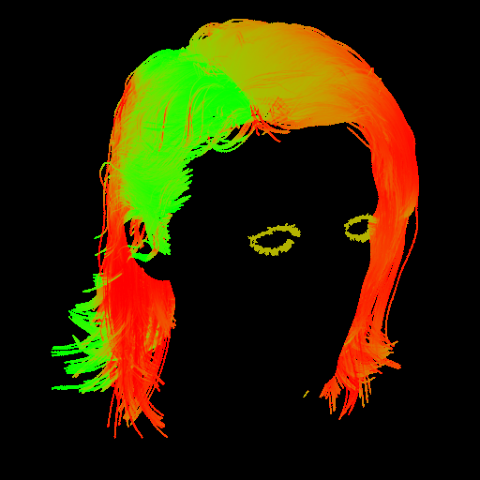
\includegraphics[width=0.11\textwidth]{project-final-paper/images/groundtruth_orientation/output_test_4.png}}
    {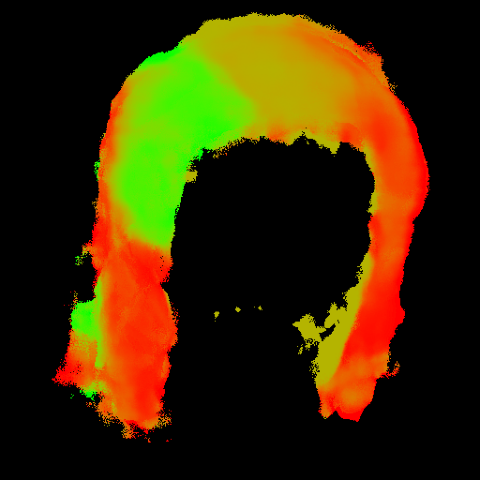
\includegraphics[width=0.11\textwidth]{project-final-paper/images/neof/output_test_4.png}}
    {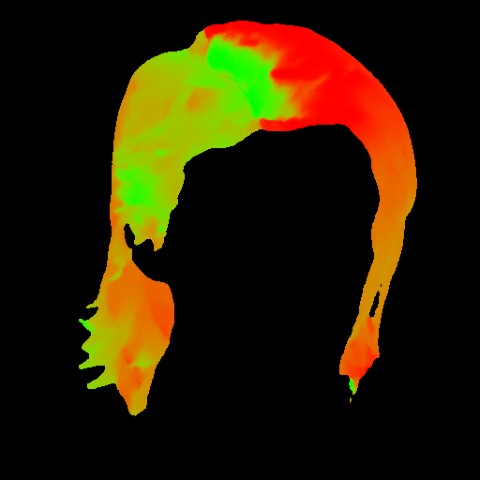
\includegraphics[width=0.11\textwidth]{project-final-paper/images/groundtruth_hairstep/output_test_4.png}}
    {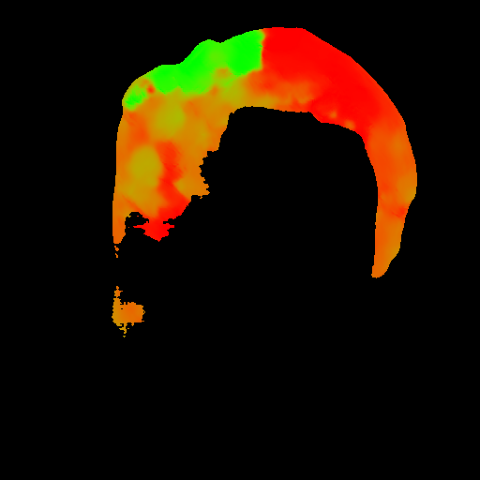
\includegraphics[width=0.11\textwidth]{project-final-paper/images/nerf_hairstep/output_test_4.png}} \\

    {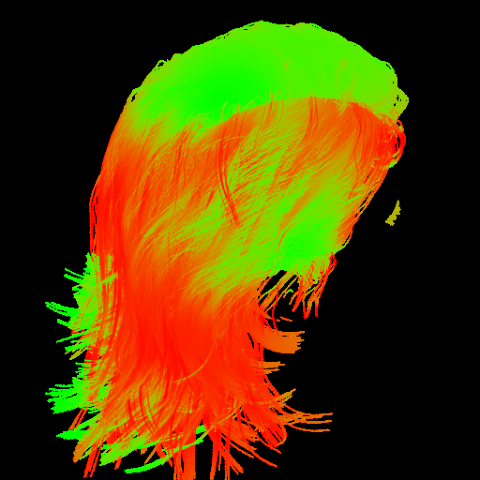
\includegraphics[width=0.11\textwidth]{project-final-paper/images/groundtruth_orientation/output_test_5.png}}
    {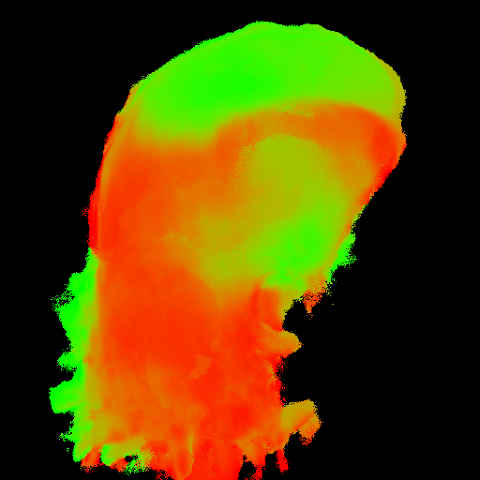
\includegraphics[width=0.11\textwidth]{project-final-paper/images/neof/output_test_5.png}}
    {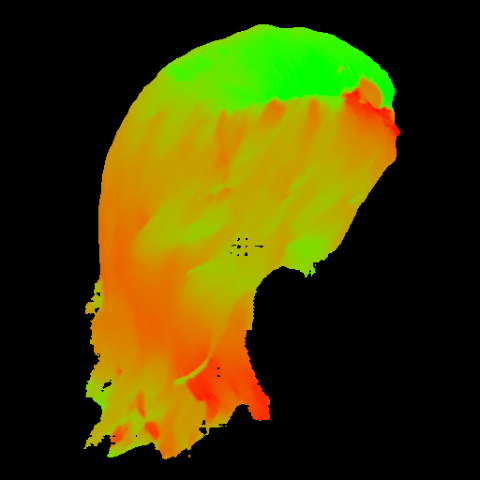
\includegraphics[width=0.11\textwidth]{project-final-paper/images/groundtruth_hairstep/output_test_5.png}}
    {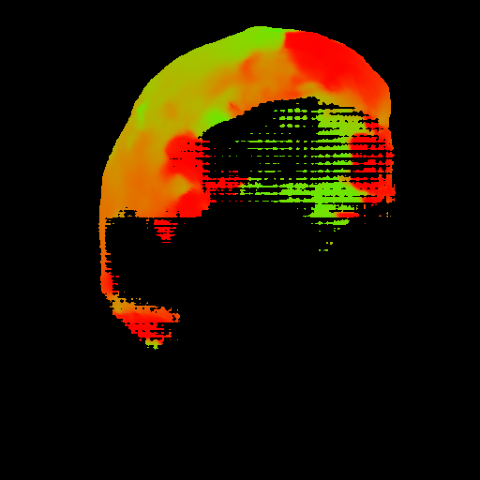
\includegraphics[width=0.11\textwidth]{project-final-paper/images/nerf_hairstep/output_test_5.png}} \\
    
    {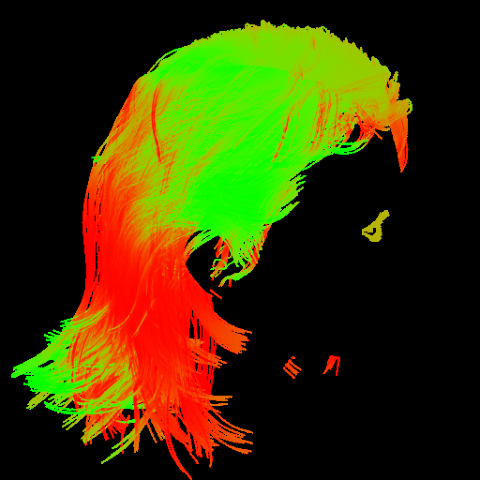
\includegraphics[width=0.11\textwidth]{project-final-paper/images/groundtruth_orientation/output_test_6.png}}
    {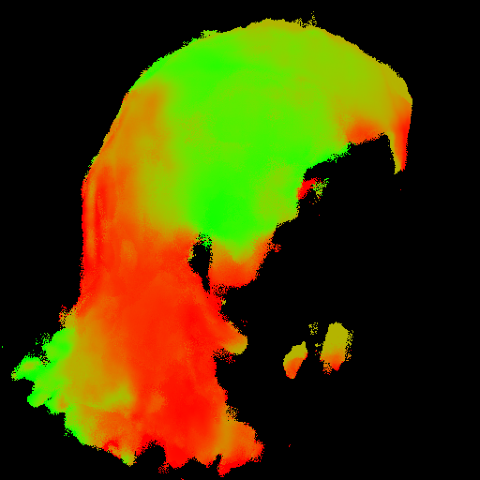
\includegraphics[width=0.11\textwidth]{project-final-paper/images/neof/output_test_6.png}}
    {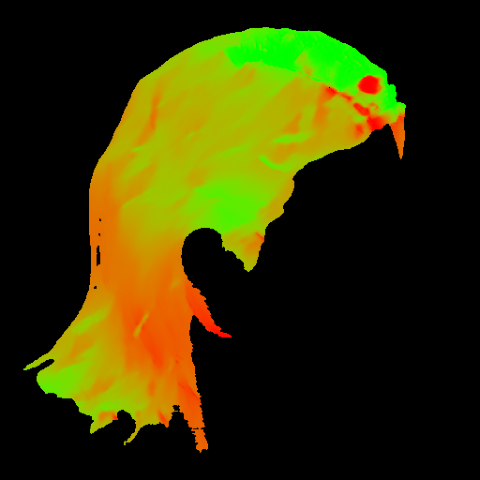
\includegraphics[width=0.11\textwidth]{project-final-paper/images/groundtruth_hairstep/output_test_6.png}}
    {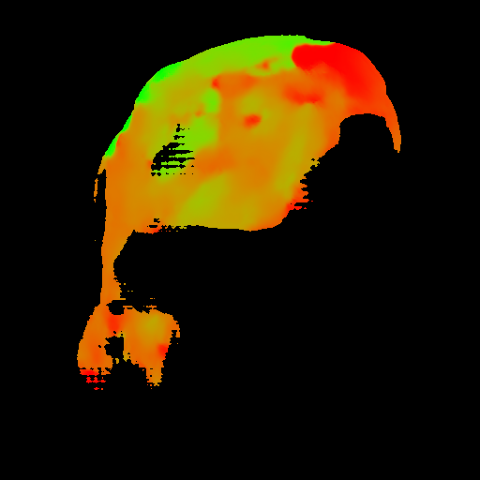
\includegraphics[width=0.11\textwidth]{project-final-paper/images/nerf_hairstep/output_test_6.png}} \\
    
     \subcaptionbox{GT}{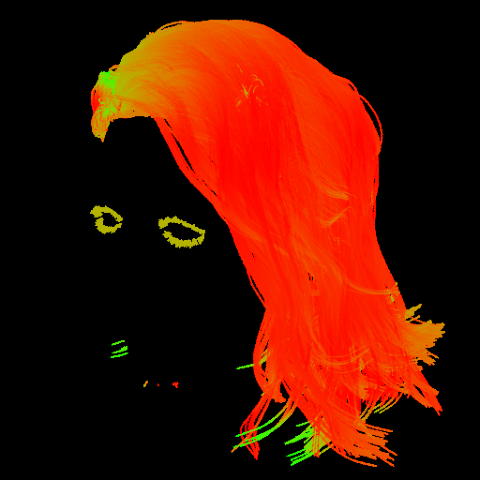
\includegraphics[width=0.11\textwidth]{project-final-paper/images/groundtruth_orientation/output_test_7.png}}
     \subcaptionbox{Ours}{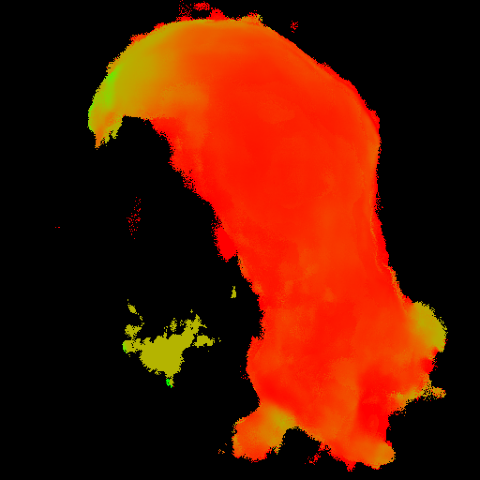
\includegraphics[width=0.11\textwidth]{project-final-paper/images/neof/output_test_7.png}}
     \subcaptionbox{HairStep}{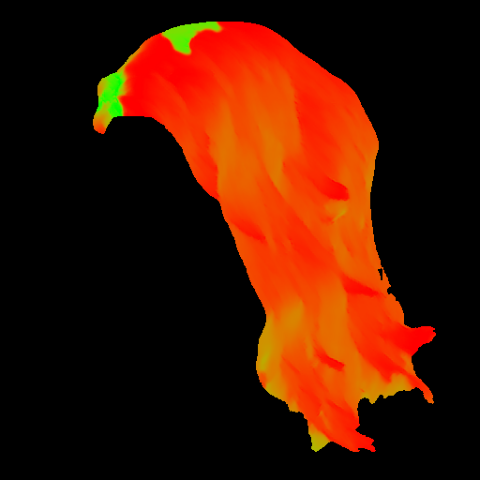
\includegraphics[width=0.11\textwidth]{project-final-paper/images/groundtruth_hairstep/output_test_7.png}}
     \subcaptionbox{NeRF}{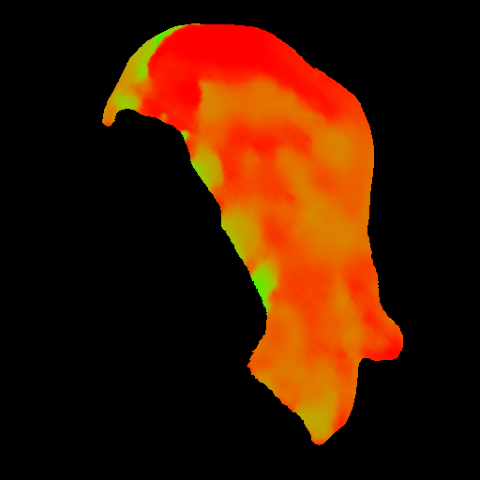
\includegraphics[width=0.11\textwidth]{project-final-paper/images/nerf_hairstep/output_test_7.png}}
    
    \caption{Normalized hair orientations, where (a) is the Ground Truth, (b) is the result our NeOF method, (c) is result of HairStep, and (d) is the result of traditional NeRF with HairStep}
    \label{fig:result_grid}
\end{figure}



\section{Conclusion}
In this paper, we propose the Neural Orientation Field (NeOF) model, which uses an MLP to implicitly encode the orientation of hair in 3D space. Compared to traditional NeRF-based or 2D image-based approaches, our method effectively reconstructs high-resolution hair growth directions with greater precision and robustness. 

Because our model can directly model the orientation field in 3D space, it enables the recovery of the entire hair direction as an editable 3D model, which allows for subsequent manual adjustments and refinements. In the future, we aim to realize a complete 3D reconstruction pipeline, enabling our method to directly output editable 3D models compatible with Blender, facilitating further editing. We believe this approach will provide a straightforward and efficient solution for sampling and automating the modeling of real human hair, significantly reducing the costs associated with traditional hair modeling in the visual effects and animation industries.

\newpage

\bibliographystyle{plainnat}
\bibliography{references}

\newpage

\section{Contribution}

\subsection{Fangjun Zhou}

COLMAP feature and camera pose preprocessing script; \texttt{colmap\_visualizer} with imagui and pyvista to help visualize the extracted point cloud/camera position; Blender camera pose extraction script and dataset generation; NeRF and NeOF camera ray generation algorithm, volumetric renderer, hierachical volume sampling, training script implementation; Introduction, related work, dataset, method, and implementation detail sections of final paper.

\subsection{Zhenyu Zhang}

Responsible for refactoring Tiny NeRF, do the training and testing related to Tiny NeRF, and implementing the code for 3D vector field reconstruction of hair growth. This included model code, loss computation code, camera view transformation and coordinate system conversion code, as well as the code of calculations for remapping 3D vectors in space to the camera frame. Also handle part of the model evaluation work, including the calculation of evaluation metrics and result visualization.

\subsection{Weiran Xu}

Contributed to building the human portrait dataset and applied HairStep for image preprocessing and hair strand direction extraction, preparing the data for analysis. Also wrote part of experiment section in the report, detailing methodology and preliminary findings.

\end{document}
